\newpage
\section{Review and Outlook}
\subsection{DiVincenzo's Criteria}
\begin{enumerate}
    \item Well defined extendible qubit array-stable memory
    \item Preparable in the ``$000\cdots$'' state
    \item Single-quantum measurements
    \item Universal set of gate operations
    \item Long decoherence time ($> 10^4$ operation time)
    \subitem And, for quantum communications,
    \item Interconvert stationary and flying qubits
    \item Transmit flying qubits from place to place
\end{enumerate}

\subsubsection{Qubits: The Building Blocks}
Qubits are physical carriers of quantum information. 

To encode a logic qubit in multiple physical qubit, we replace $\ket{0}$ and $\ket{1}$ by the codewords, e.g., in the 3-qubit repetition code,
\begin{align*}
    \ket{\tilde{0}}=\ket{0}\ket{0}\ket{0}=\ket{000},\ \ket{\tilde{1}}=\ket{1}\ket{1}\ket{1}=\ket{111}
\end{align*}

In the 2D complex vector space, any Hermitian operator $\hat{n}\cdot \vec{\sigma}$, where $\hat{n}=$ can be expressed as 
\begin{align*}
    \hat{O}=d\hat{I}+a\hat{\sigma}_x+b\hat{\sigma}_y+c\hat{\sigma}_z
\end{align*}
where $a,b,c,d\in\mathbb{R}$. 

Pauli matrices $\hat{\sigma}_{x,y,z}$ satisfy the following relations:
\begin{align*}
    \hat{\sigma}_x^2&=\hat{\sigma}_y^2=\hat{\sigma}_z^2=1\\
    \hat{\sigma}_x\hat{\sigma}_y&=-\hat{\sigma}_y\hat{\sigma}_x=i\hat{\sigma}_z\\
    \hat{\sigma}_y\hat{\sigma}_z&=-\hat{\sigma}_z\hat{\sigma}_y=i\hat{\sigma}_x\\
    \hat{\sigma}_z\hat{\sigma}_x&=-\hat{\sigma}_x\hat{\sigma}_z=i\hat{\sigma}_y
\end{align*}

We can further defnie 
\begin{align*}
    \hat{\sigma}_+=\frac{\hat{\sigma}_x+i\hat{\sigma}_y}{2},\ \hat{\sigma}_-=\frac{\hat{\sigma}_x-i\hat{\sigma}_y}{2}
\end{align*}
Therefore, we have
\begin{align*}
    \hat{\sigma}_z\ket{g}&=\ket{g},\ \hat{\sigma}_z\ket{e}=-\ket{e}\\
    \hat{\sigma}_+\ket{g}&=\ket{e},\ \hat{\sigma}_-\ket{e}=\ket{g}
\end{align*}
where our convention is $\ket{g}\equiv\ket{0}$ and $\ket{e}\equiv\ket{1}$. For a logical qubit, operators are typically the products of a string of physical spin operators. 

A quantum harmonic oscillator (QHO) is defined by energy eigenstates 
\begin{align*}
    \left\{ \ket{n}:E_n=\left( n+\frac{1}{2} \right)\hbar \omega_c,\ n=0,1,2,\dots \right\}
\end{align*} 
and a pair of ladder operators $a, a^\dagger$ that satisfy
\begin{align*}
    a\ket{n}&=\sqrt{n}\ket{n-1},\ a^\dagger\ket{n}=\sqrt{n+1}\ket{n+1}\\
    [a, a^\dagger]&\equiv aa^\dagger-a^\dagger a=1
\end{align*}
A transmon qubit is a QHO with a small anharmonicity
\begin{align*}
    \hat{H}_{tr}=4E_C\hat{n}^2-E_J\cos\hat{\varphi}\approx 4E_C\hat{n}^2+\frac{1}{2}E_J\hat{\varphi}^2
\end{align*}
where $E_C=\frac{e^2}{2C}$ and $E_J=\frac{\hbar^2}{4e^2 L}$

\begin{figure}[!htb]
    \centering
    \includegraphics[width=0.309\textwidth]{pic/Review/the qubit is insensitive to charge fluctuation.png}
    \caption{As the result of large $\frac{E_J}{E_C}$ , the qubit is insensitive to charge fluctuation}
\end{figure}


\subsubsection{A Variety of States}
A generic pure state of a qubit is 
\begin{align*}
    \ket{\psi}=\alpha\ket{0}+\beta\ket{1}=\begin{pmatrix}
        \alpha\\ \beta
    \end{pmatrix}
\end{align*}
$\alpha,\beta\in \mathbb{C}$, normalized by 
\begin{align*}
    \braket{\psi|\psi}=|\alpha|^2+|\beta|^2=1
\end{align*}

A pure single-qubit state can represented by a point on the Bloch sphere:
\begin{align*}
    \ket{\psi}=\cos\frac{\theta}{2}\ket{0}+e^{i\phi}\sin\frac{\theta}{2}\ket{1}
\end{align*}

\begin{figure}[!htb]
    \centering
    \includegraphics[width=0.309\textwidth]{pic/Review/the Bloch sphere.png}
    \caption{the Bloch sphere}
\end{figure}


The state is an eigenvector of the operator $\hat{n}\cdot \vec{\sigma}$, where $\hat{n}=(\sin\theta\cos\phi,\ \sin\theta\sin\phi,\ \cos\theta)$ points to the representative point on the Bloch sphere. 


Density matrices in the form of $\rho=\sum_i P_i\ket{\psi_i}\bra{\psi_i}$ (with $\sum_i P_i=1$) can describe both pure and mixed states.

The key properties of density matrices are:
\begin{enumerate}
    \item Density matrices are Hermitian $\rho_{ij}=\bar{\rho}_{ji}$
    \item The trace of a density matrix is 1 $\mathrm{Tr}(\rho)=1$
    \item The eigenvalues of the density matrix are all positive and lie bewteen 0 and 1.
\end{enumerate}
For a pure state
\begin{align*}
    \rho^2=\rho,\ \mathrm{Tr}(\rho^2)=1
\end{align*}
For a mixed state (or a subsystem of an entangled state)
\begin{align*}
    \rho^2\ne \rho,\ \mathrm{Tr}(\rho^2)<1
\end{align*}

In a combined system ($\mathcal{H} =\mathcal{H}_A\otimes\mathcal{H}_B$), a quantum state can be separable, i.e.$\ket{\Psi}=\ket{\phi}_A\otimes\ket{\psi}_B$. Its reduced density matrix (约化密度矩阵), say $\rho_A=\mathrm{Tr}_B(\rho)$, satisfies
\begin{align*}
    \rho_A^2=\rho_A,\ \mathrm{Tr} \rho_A^2=1
\end{align*}

More interestingly, a state can be entangled, i.e., $\mathrm{Tr}\rho_A^2<1$. It encodes nontrivial mutual information, measurable by entanglement entropy(纠缠熵)
\begin{align*}
    S_A\equiv -\mathrm{Tr}_A(\rho_A\log_2\rho_A)>0
\end{align*}

The well-known maximally entangled states are the Bell states, which can be distinguished and stabilized by $X_1X_2$ and $Z_1Z_2$. 

\begin{table}[!htb]
    \centering
    \caption{Bell states}
    \begin{tabular}[c]{ccc}\toprule
        Bell States & $X_1X_2$ & $Z_1Z_2$\\ \midrule
        $\ket{\Psi_{00}}=\frac{\ket{00}+\ket{11}}{\sqrt{2}}$ & $+1$ & $+1$ \\
        $\ket{\Psi_{01}}=\frac{\ket{01}+\ket{10}}{\sqrt{2}}$ & $+1$ & $-1$ \\
        $\ket{\Psi_{10}}=\frac{\ket{00}-\ket{11}}{\sqrt{2}}$ & $-1$ & $+1$ \\
        $\ket{\Psi_{11}}=\frac{\ket{01}-\ket{10}}{\sqrt{2}}$ & $-1$ & $-1$ 
        \\ \bottomrule
    \end{tabular}
\end{table}

It's not possible to perfectly clone an unknown quantum state, or a state drawn from a set of tow (or more) non-orthogonal states (quantum no-cloning theorem)(反证此定理). In other words, it's impossible to unitary evolve
\begin{align*}
    \ket{\psi}\ket{0}\rightarrow\ket{\psi}\ket{\psi}
\end{align*}
for an unknown $\ket{\psi}$ even with any environment. 

Meanwhile, the following evolution is frequently used in quantum computation and quantum communication. (纠缠)
\begin{align*}
    (\alpha\ket{0}+\beta\ket{1})\ket{0}\xrightarrow{CNOT} \alpha\ket{00}+\beta\ket{11}
\end{align*}

\subsubsection{Gates: Controlling the State of Qubits}
Given the state of a system $\ket{\psi(0)}$ at time $t=0$, the state of the system at time $t$ can be expressed as 
\begin{align*}
    \ket{\psi(t)}=U(t)\ket{\psi(0)}
\end{align*}
where $U(t)$ is called the time-evolution operator. 

For time-independent Hamiltonian $H$, we have symbolically
\begin{align*}
    U(t)=e^{-iHt/\hbar}
\end{align*}
which leads to Schroedinger's equation
\begin{align*}
    i\hbar\frac{\partial \ket{\psi(t)}}{\partial t}=H\ket{\psi(t)}
\end{align*}

Such a unitary evolution is reversible operation(演化可逆). 

For universal quantum computation(完备门集), we only need a small set of single-qubit gates and a two-qubit gate. 

A practical scheme to control and entangle superconducting qubits is to couple them to microwave resonators, whose single EM-field mode is a QHO. This research field is known as circuit QED. 

To simplify, the coupled system can often be thought of as two qubits interacting with 
\begin{align*}
    H_{int}=J_x\sigma_x^{(1)}\sigma_x^{(2)}+J_y\sigma_y^{(1)}\sigma_y^{(2)}+J_z\sigma_z^{(1)}\sigma_z^{(2)}
\end{align*}
Understanding the time evolution under $H_{int}$ is important to the design of a two-qubit quantum gate.

\subsubsection{Entangled with Measuring Apparatuses}
If $\ket{\psi}$ is the state-vector of a quantum system, and the observable $L$ is measured, the probability to observe the eigenvalue $\lambda$ is 
\begin{align*}
    P_\lambda=\braket{\psi|\lambda}\braket{\lambda|\psi}
\end{align*}
where $\ket{\lambda}$ is the corresponding eigenvector. (算符代表潜在的值, 态是测出来的几率)

The state of the system immediately after the measurement is 
\begin{align*}
    \frac{\ket{\lambda}\braket{\lambda|\psi}}{\sqrt{P_\lambda}}
\end{align*}

State and measurement in the quantum world are two different things. Non-orthogonal (non-identical, hence different) states cannot be reliably distinguished. (测量与态并不是一回事)

In the statistical sense, the experimental average is identical to the expectation value of $M$ of the system (测量均值)
\begin{align*}
    \braket{M}\equiv \braket{\psi|M|\psi},\ \text{ or }\mathrm{Tr}\rho M
\end{align*}
The uncertainty of the measurement is understood as the standard deviation $\Delta M=\sqrt{\braket{M^2}-\braket{M}^2}$ of the results measured from a large nunmberof quantum systems in identical states. 

The quantum circuit model for a measurement of an operator $U$ acting on a single qubit is

\begin{figure}[!htb]
    \centering
    \begin{quantikz}
        \lstick{$\ket{0}$}&\gate{H}&\ctrl{1}&\gate{H}&\meter{}&\\
        \lstick{$\alpha\ket{u_+}+\beta\ket{u_-}$}& & \gate{U} & & &
    \end{quantikz}
\end{figure}
Here, we suppose $U$ has eigenvalues $\pm 1$ and corresponding eigenvector $\ket{u_\pm}$. The data qubit and the measurement qubit are generically
entangled in the state $\alpha\ket{0}\ket{u_+}+\beta\ket{1}\ket{u_-}$ before the projective measurement. 

\subsubsection{Decoherence: The Environment Issues}
To study the combined evolution of system ($S$) and its environment ($E$), we start from a separable density matrix
\begin{align*}
    \rho=\rho_s(0)\otimes\rho_E(0)
\end{align*}
In particular, we can write
\begin{align*}
    \rho_E(0)=\ket{0}\bra{0}
\end{align*}
where $\ket{0}$ belongs to a set of environment orthogonal basis states $\ket{i}$. 

Given a unitary time evolution operator $U(t)$ for the total system, the evolution of the reduced density matrix is captured by the Kraus operators $E_i=\braket{i|U(t)|0}$:
\begin{align*}
    \rho_S(t)&=Tr_E\left\{ U(t)[\rho_S(0)\otimes \ket{0}\bra{0}]U^\dagger (t) \right\}\\
    &=\sum_iE_i\rho_S(0)E_i^\dagger
\end{align*}
The effects of noise are usually separated into relaxation (qubit flip)(激发态$\rightarrow$基态) and dephasing (phase randomization)(能级的能量差变化导致相位变化). (整体都称为退相干)

The energy dissipation is described by amplitude damping with
\begin{align*}
    E_0\begin{pmatrix}
        1 & 0\\ 0& \sqrt{1-p}
    \end{pmatrix},\ E_1=\begin{pmatrix}
        0 & \sqrt{p}\\  0 & 0
    \end{pmatrix}
\end{align*}

The loss of quantum information without loss of energy is described by phase damping (e.g., when a photon scatters randomly as it travels through a waveguide) with
\begin{align*}
    E_0\begin{pmatrix}
        1 & 0\\ 0& \sqrt{1-p}
    \end{pmatrix},\ E_1=\begin{pmatrix}
        0 & 0\\  0 & \sqrt{p}
    \end{pmatrix}
\end{align*}

\subsection{The Era of NISQ Computers}
They are systems that have up to thousands of qubits or even more but not full error-correction, thus noisy. They fit the term of noisy intermediate-scale quantum (NISQ) computers.

\subsubsection{Quantum Algorithms}
\paragraph{Grover's algorithm}
Grover’s algorithm searches for an entry in an unstructured database and, thus, can be practically useful. Geometrically, the algorithm rotates a state toward the target through a series of reflections. One can show that the number of search steps goes from $O(N)$ to $O(\sqrt{N})$. If we run the algorithm once, we only have a very high probability to obtain the desired result. To ensure the success, we need to repeat the computation a few times.

\begin{figure}[htb]
    \centering
    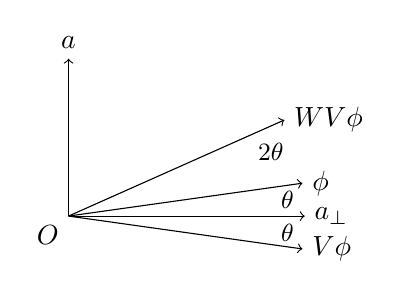
\begin{tikzpicture}
        \draw [->] (0, 0)--(0, 2) node[above] {$\ket{a}$};
        \draw [->] (0, 0)--(3, 0) node[right] {$\ket{a_\perp}$};
        \draw [->] (0, 0)--(8:3) node[right] {$\ket{\phi}$};
        \draw [->] (0, 0)--(-8:3) node[right] {$V\ket{\phi}$};
        \draw [->] (0, 0)--(24:3) node[right] {$WV\ket{\phi}$};
        \node at (0, 0) [below left] {$O$};

        \path (-8:3) -- node[midway,left] {\small$\theta$} (0:3);
        \path (8:3) -- node[midway,left] {\small$\theta$} (0:3);
        \path (8:3) -- node[midway, left] {\small$2\theta$} (24:3);
    \end{tikzpicture}
\end{figure}

We choose
\begin{align*}
    \ket{\phi}=H^{\otimes n}\ket{0}_n=\frac{1}{2^{n/2}}\sum_{x=0}^{2^n-1}\ket{x}_n
\end{align*}
Reflection $V$ with respect to the direction of $\ket{a_\perp}$ is 
\begin{align*}
    V=2\ket{a_\perp}\bra{a_\perp}-I=I-2\ket{a}\bra{a}
\end{align*}
Reflection $W$ with respect to $\ket{\phi}$ is
\begin{align*}
    W=2\ket{\phi}\bra{\phi}-I
\end{align*}
The product of the two reflections is a rotation: $WV$ rotates a vector through the angle $2\theta$. (如何计算需要转多少次)

\subsubsection{Quantum Error Correction}
(测量不相干信息进行探测纠正错误)(编码信息, 测量其是否仍在编码空间, 若不在纠正之)
%P31 fig
In the three-qubit repetition code, we measure two stabilizer generators $U_1=Z_1Z_2$ and $U_2=Z_2Z_3$. 

\begin{figure}[!htb]
    \centering
    \includegraphics[width=0.309\textwidth]{pic/Review/the three-qubit repetition code}
    \caption{the three-qubit repetition code}
\end{figure}

The operators $U_1$ and $U_2$ each has two distinct eigenvalues $\pm1$. The measurement of the operators, for zero and one-qubit errors, yields
\begin{table}[htb]
    \centering
    \begin{tabular}[c]{ccccc}\toprule
        & $I$ & $X_1$ & $X_2$ & $X_3$\\ \midrule
        $U_1=Z_1Z_2$ & $+1$ & $-1$ & $-1$ & $+1$\\ 
        $U_2=Z_2Z_3$ & $+1$ & $+1$ & $-1$ & $-1$\\ \bottomrule
    \end{tabular}
\end{table}
Therefore, the measurement results allows us to correct a single bit-flip error.


%P33 fig
Surface code(容错量子计算)is a possible fault-tolerant encoding scheme. Errors can be detected by the change of measurement results. Sufficiently rare errors can be left uncorrected and undone in classical control software.

\begin{figure}[!htb]
    \centering
    \includegraphics[width=0.309\textwidth]{pic/Review/Surface code}
    \caption{Surface code}
\end{figure}


\subsection{Calculation}
\subsubsection{Tensor product}
\begin{align*}
    \mathcal{H}&\rightarrow\mathcal{H}^1\otimes \mathcal{H}^2\\
    \ket{0}, \ket{1}&\rightarrow \ket{00}, \ket{01}, \ket{10}, \ket{11}
\end{align*}

\begin{align*}
    H&=\sum \vec{\sigma}_1\vec{\sigma}_2=\sum(\sigma_1^x\sigma_2^x+\sigma_1^y\sigma_2^y+\sigma_1^z\sigma_2^z)
\end{align*}
只会有$2\times2$的矩阵分解 
\begin{align*}
    H&=aI+b\sigma_x+c\sigma_y+d\sigma_d\\
    &=\begin{pmatrix}
        d & b-ic\\
        b+ic & a
    \end{pmatrix}\\
    &=B\hat{n}\vec{\sigma}\\
    E_\pm&=a\pm\sqrt{b^2+c^2+d^2}
\end{align*}

\begin{table}[H]
    \centering
    \caption{$\sigma\rightarrow H$}
    \begin{tabular}[c]{cccc}
        00 & 01 & 10 & 11\\
    \end{tabular}
\end{table}


\subsubsection{partial trace}
\begin{align*}
    \ket{\psi}&=\frac{1}{\sqrt{1}}\ket{00}+\frac{1}{\sqrt{2}}\ket{11}\\
    \rho&=\ket{\psi}\bra{\psi}\\
    \rho_A&=Tr_B\rho={}_B\braket{0|\rho|0}_B+{}_B\braket{1|\rho|1}_B\\
    &=\frac{1}{2}\ket{0}\bra{0}+\frac{1}{2}\ket{1}\bra{1}
\end{align*}


\begin{align*}
    \braket{k|U|0}->E_k
\end{align*}

\subsubsection{\texorpdfstring{$e^{-iHt}$}.}
\begin{align*}
    H&=\\
    e^{-iHt}&=\sum_i\frac{(-it)^jH^j}{j!}
\end{align*}




\subsubsection{Qubit Gate}
单比特门 $2\times 2$
\begin{align*}
    \ket{\psi_{out}}=U\ket{\psi_{in}}
\end{align*}

双bite门 $4\times 4$
\begin{align*}
    \ket{\psi_{out}^{(2)}}=U\ket{\psi_{in}^{(2)}}
\end{align*}

\paragraph{Ctrl-Z}

\begin{align*}
    \begin{pmatrix}
        1 & & &\\
        &1& &\\
        & &1&\\
        & & &-1\\
    \end{pmatrix}
\end{align*}

\paragraph{Swap}
\begin{align*}
    \begin{pmatrix}
        1 &   &   &   \\
          &   & 1 &   \\
          & 1 &   &   \\
          &   &   & 1 \\
    \end{pmatrix}
\end{align*}

\paragraph{\texorpdfstring{$\sqrt{i Swap}$}.}

\begin{align*}
    \begin{pmatrix}
        1 &   &   &   \\
          &   & 1 &   \\
          & 1 &   &   \\
          &   &   & 1 \\
    \end{pmatrix}
\end{align*}